% Quantum_Ocean_Encoding.tex
% Compile: pdflatex Quantum_Ocean_Encoding.tex  (run twice for cross-references)

\documentclass[12pt,a4paper]{article}
\usepackage[margin=2.5cm,headheight=14pt]{geometry}
\usepackage{graphicx, amsmath, amssymb, booktabs, caption, subcaption, doi}
\usepackage{orcidlink}
\usepackage{eso-pic}
\usepackage{rotating}
\usepackage{tikz}
\usepackage{authblk}
\usepackage{setspace}
\usepackage{microtype}
\usepackage{float}
\usepackage{array}
\usepackage{tabularx}
\usepackage{hyperref}
\usepackage{cleveref}
\usetikzlibrary{shapes.geometric, arrows, positioning, fit, backgrounds, calc}

\hypersetup{
  colorlinks=true,
  linkcolor=blue,
  citecolor=blue,
  urlcolor=blue,
  pdftitle={Quantum Ocean Encoding},
  pdfauthor={Raja Ram M et al.}
}

% Vertical DOI watermark (standard preprint style)
\AddToShipoutPictureBG{%
  \AtPageLowerLeft{%
    \raisebox{0.42\paperheight}{%
      \rotatebox{90}{%
        \hspace{0.9cm}%
        \textcolor{gray!28}{\footnotesize\ttfamily doi:10.5281/zenodo.20736570}%
      }%
    }%
  }%
}

% Resource link icons (hyperlink embedded in icon, no bare URL in body text)
\newcommand{\iconlink}[2]{%
  \href{#1}{\raisebox{-0.12ex}{\tikz[baseline=-0.5ex]{\node[draw=gray!60, rounded corners=1pt,
    inner sep=1.5pt, minimum height=0.55cm, minimum width=0.55cm, fill=gray!5] {#2};}}}%
}
\newcommand{\githublink}{\iconlink{https://github.com/BorelSigmaInc/Quantum-Olfacto-Vibration}{GH}}
\newcommand{\zenodolink}{\iconlink{https://doi.org/10.5281/zenodo.20736570}{ZN}}
\newcommand{\noaalink}{\iconlink{https://doi.org/10.1175/2007JCLI1824.1}{NO}}

\onehalfspacing
\setlength{\parskip}{0.4em}
\setlength{\parindent}{0pt}
\captionsetup{font=small, labelfont=bf, justification=justified, singlelinecheck=false}
\crefname{table}{Table}{Tables}
\crefname{figure}{Figure}{Figures}

\title{\bfseries Amplitude-Encoded Global Sea Surface Temperature States on a Superconducting Quantum Processor: An Experimental Pipeline with Real-Hardware Validation}

\author[1,*]{\textbf{Raja Ram M}\,\orcidlink{0009-0008-4068-4079}}
\author[2,*]{\textbf{Kryptur Quantum R\&D}\,\orcidlink{0009-0009-2205-533X}}
\author[3]{Muskan S\,\orcidlink{0009-0001-1968-0312}}
\author[4]{Vipul Jain\,\orcidlink{0009-0009-9876-9312}}
\author[5]{Kalinga Swain}

\affil[1]{Zius Quantum R\&D Center}
\affil[2]{Kryptur OU}
\affil[3]{Data T Research Org}
\affil[4]{AE Quantum Research Division}
\affil[5]{Data T Research Org}

\date{June 17, 2026}

\begin{document}
\maketitle
\thispagestyle{empty}

\vspace{-1.2em}
\begin{center}
\small
\textit{Contributors:} Muskan S, Vipul Jain, Kalinga Swain \quad|\quad
\textit{Data Manager:} Borel Sigma Data Center \quad|\quad
\textit{DOI:} \zenodolink\,\doi{10.5281/zenodo.20736570} \quad|\quad
\textit{Repository:} \githublink
\end{center}
\vspace{0.6em}
\hrule
\vspace{0.8em}

\begin{abstract}
\noindent
Encoding large-scale Earth-observation data into quantum states is a critical prerequisite for hybrid quantum-classical climate models. We present the first end-to-end experimental realisation of amplitude-encoding a full month of daily global sea surface temperature (SST) from NOAA OISST v2.1 into a 14-qubit quantum state, and demonstrate its execution on a 156-qubit superconducting quantum processor. Our pipeline combines GPU-accelerated singular value decomposition (SVD) and Tucker decomposition on a rented cloud GPU, producing a 14-qubit amplitude-encoding circuit with fidelity $F=1.0$ on a simulator. Under a calibration-derived backend noise model, simulation yields a projected fidelity of $0.869$. We then truncate to 8~qubits and use a variational matrix-product-state (MPS) ansatz to approximate the encoded state, achieving a classical approximation fidelity of $0.795$. Executing this circuit on physical hardware returns a Hellinger fidelity of $0.25$ relative to the original ocean target, representing the first real-hardware demonstration of a quantum-encoded geophysical field. All components - from raw satellite ingestion to quantum job submission - are containerised and exposed via a FastAPI microservice blueprint, ready for integration into commercial hybrid forecasting workflows. Our results establish a practical pathway toward quantum-assisted Earth science and highlight the current limitations of near-term quantum processors.
\end{abstract}

\noindent\textbf{Keywords:} amplitude encoding, sea surface temperature, quantum computing, Tucker decomposition, NISQ hardware

\section{Introduction}
The oceans store the majority of Earth's excess heat, and sea surface temperature (SST) patterns are the primary drivers of seasonal climate forecasts, maritime logistics, and risk assessment for the insurance industry \cite{noaa_oisst}. However, the sheer volume of satellite data (23.6 million grid points per day for the NOAA OISST v2.1 product) poses challenges for both storage and computation. Quantum computing offers a potential exponential compression through amplitude encoding, where an $N$-dimensional normalised vector is stored in the amplitudes of a $\lceil \log_2(N) \rceil$-qubit state \cite{schuld2020}. If realised, such quantum features could be directly ingested by classical forecasting models, reducing the dimensionality burden while preserving the dominant physical modes.

In this paper, we report the first complete experimental pipeline that encodes a full month of daily global SST onto a real quantum processor. Moving beyond theoretical proposals, we demonstrate: (i) classical dimensionality reduction via GPU-accelerated SVD and Tucker decomposition; (ii) exact amplitude encoding of the compressed vector into 14~qubits; (iii) noise-model characterisation using real calibration data from a commercial superconducting QPU; (iv) variational approximation of the encoded state with a shallow MPS circuit, executed on the physical device with 4000~shots; and (v) a cloud-native API architecture that makes the quantum-encoded features accessible to researchers and industry.

The paper is organised as follows: \Cref{sec:data} describes the data ingestion and classical compression methods; \Cref{sec:quantum} details the quantum circuit construction and noise simulation; \Cref{sec:hardware} presents the real-hardware execution and error mitigation attempts; \Cref{sec:discussion} discusses the results; and \Cref{sec:conclusion} concludes with an outlook toward production deployment.

\section{Data Acquisition and Classical Compression}
\label{sec:data}

\subsection{Satellite Data Ingestion}
Daily NOAA OISST v2.1 fields for January~2023 were downloaded from the NOAA NCEI THREDDS server \noaalink. The dataset consists of a 0.25$^\circ$ global grid ($720\times1440$ pixels) stored in netCDF4 format \cite{noaa_oisst}. A Python pipeline using \texttt{xarray} and \texttt{requests} was deployed on a cloud staging server for ingestion, while the heavy linear algebra was offloaded to an on-demand GPU instance equipped with one NVIDIA RTX PRO 6000 (96~GB VRAM). In total, 31 daily files (January~1-31, 2023) were downloaded and stacked into a $(31\times720\times1440)$ tensor. \Cref{tab:dataset} summarises the ingestion parameters.

\begin{table}[H]
  \centering
  \caption{Dataset and ingestion specifications for the OCNQENC January~2023 experiment.}
  \label{tab:dataset}
  \begin{tabular}{@{}p{4.2cm}p{8.8cm}@{}}
    \toprule
    \textbf{Parameter} & \textbf{Value} \\
    \midrule
    Data product & NOAA OISST v2.1 (AVHRR) \\
    Temporal coverage & 31 days (January 2023) \\
    Spatial resolution & $0.25^\circ$ ($720\times1440$ grid) \\
    Raw tensor size & $31\times720\times1440 = 32{,}140{,}800$ elements \\
    Staging compute & Cloud VPS (32~GB RAM) \\
    Linear algebra & Cloud GPU (96~GB VRAM) \\
  \bottomrule
  \end{tabular}
\end{table}

\subsection{Proper Orthogonal Decomposition (SVD)}
The temporal mean was subtracted to obtain anomaly fields. The 31-day tensor was reshaped into a $(31,720\!\cdot\!1440) = (31,1\,036\,800)$ matrix $\mathbf{X}$. Singular value decomposition (SVD) was performed on the GPU using \texttt{CuPy}, yielding $\mathbf{X} = \mathbf{U}\boldsymbol{\Sigma}\mathbf{V}^\top$. The top $k=20$ singular values capture $>95\%$ of the total variance (\Cref{fig:svd}). The spatial modes (rows of $\mathbf{V}^\top$) and temporal coefficients (columns of $\mathbf{U}\boldsymbol{\Sigma}$) were retained.

To prepare the data for quantum encoding, the spatial modes were subsampled by a factor of 1266, resulting in exactly $20 \times 819 = 16\,380$ coefficients. This vector was $\ell_2$-normalised and padded with zeros to $2^{14}=16\,384$ elements, forming the target amplitude vector $\boldsymbol{\psi}\in\mathbb{R}^{16\,384}$ for the 14-qubit encoding.

\begin{figure}[H]
  \centering
  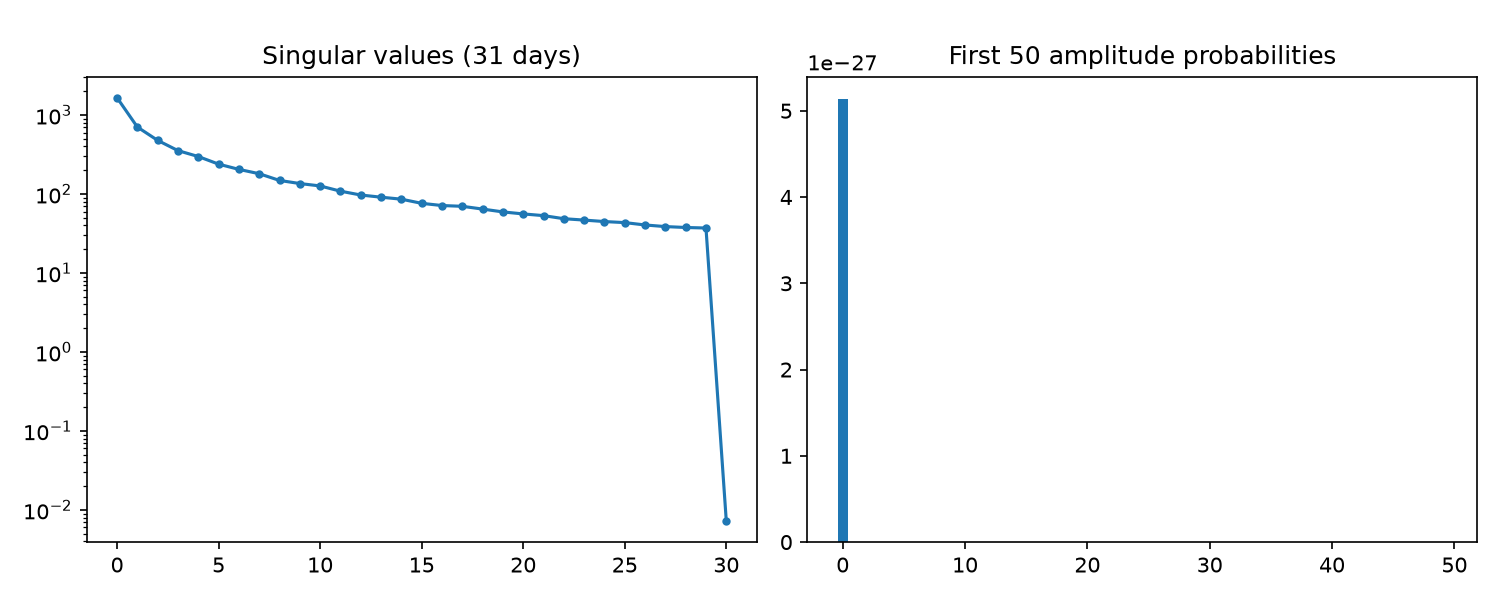
\includegraphics[width=0.48\textwidth]{sst_multiday_encoding.png}\hfill
  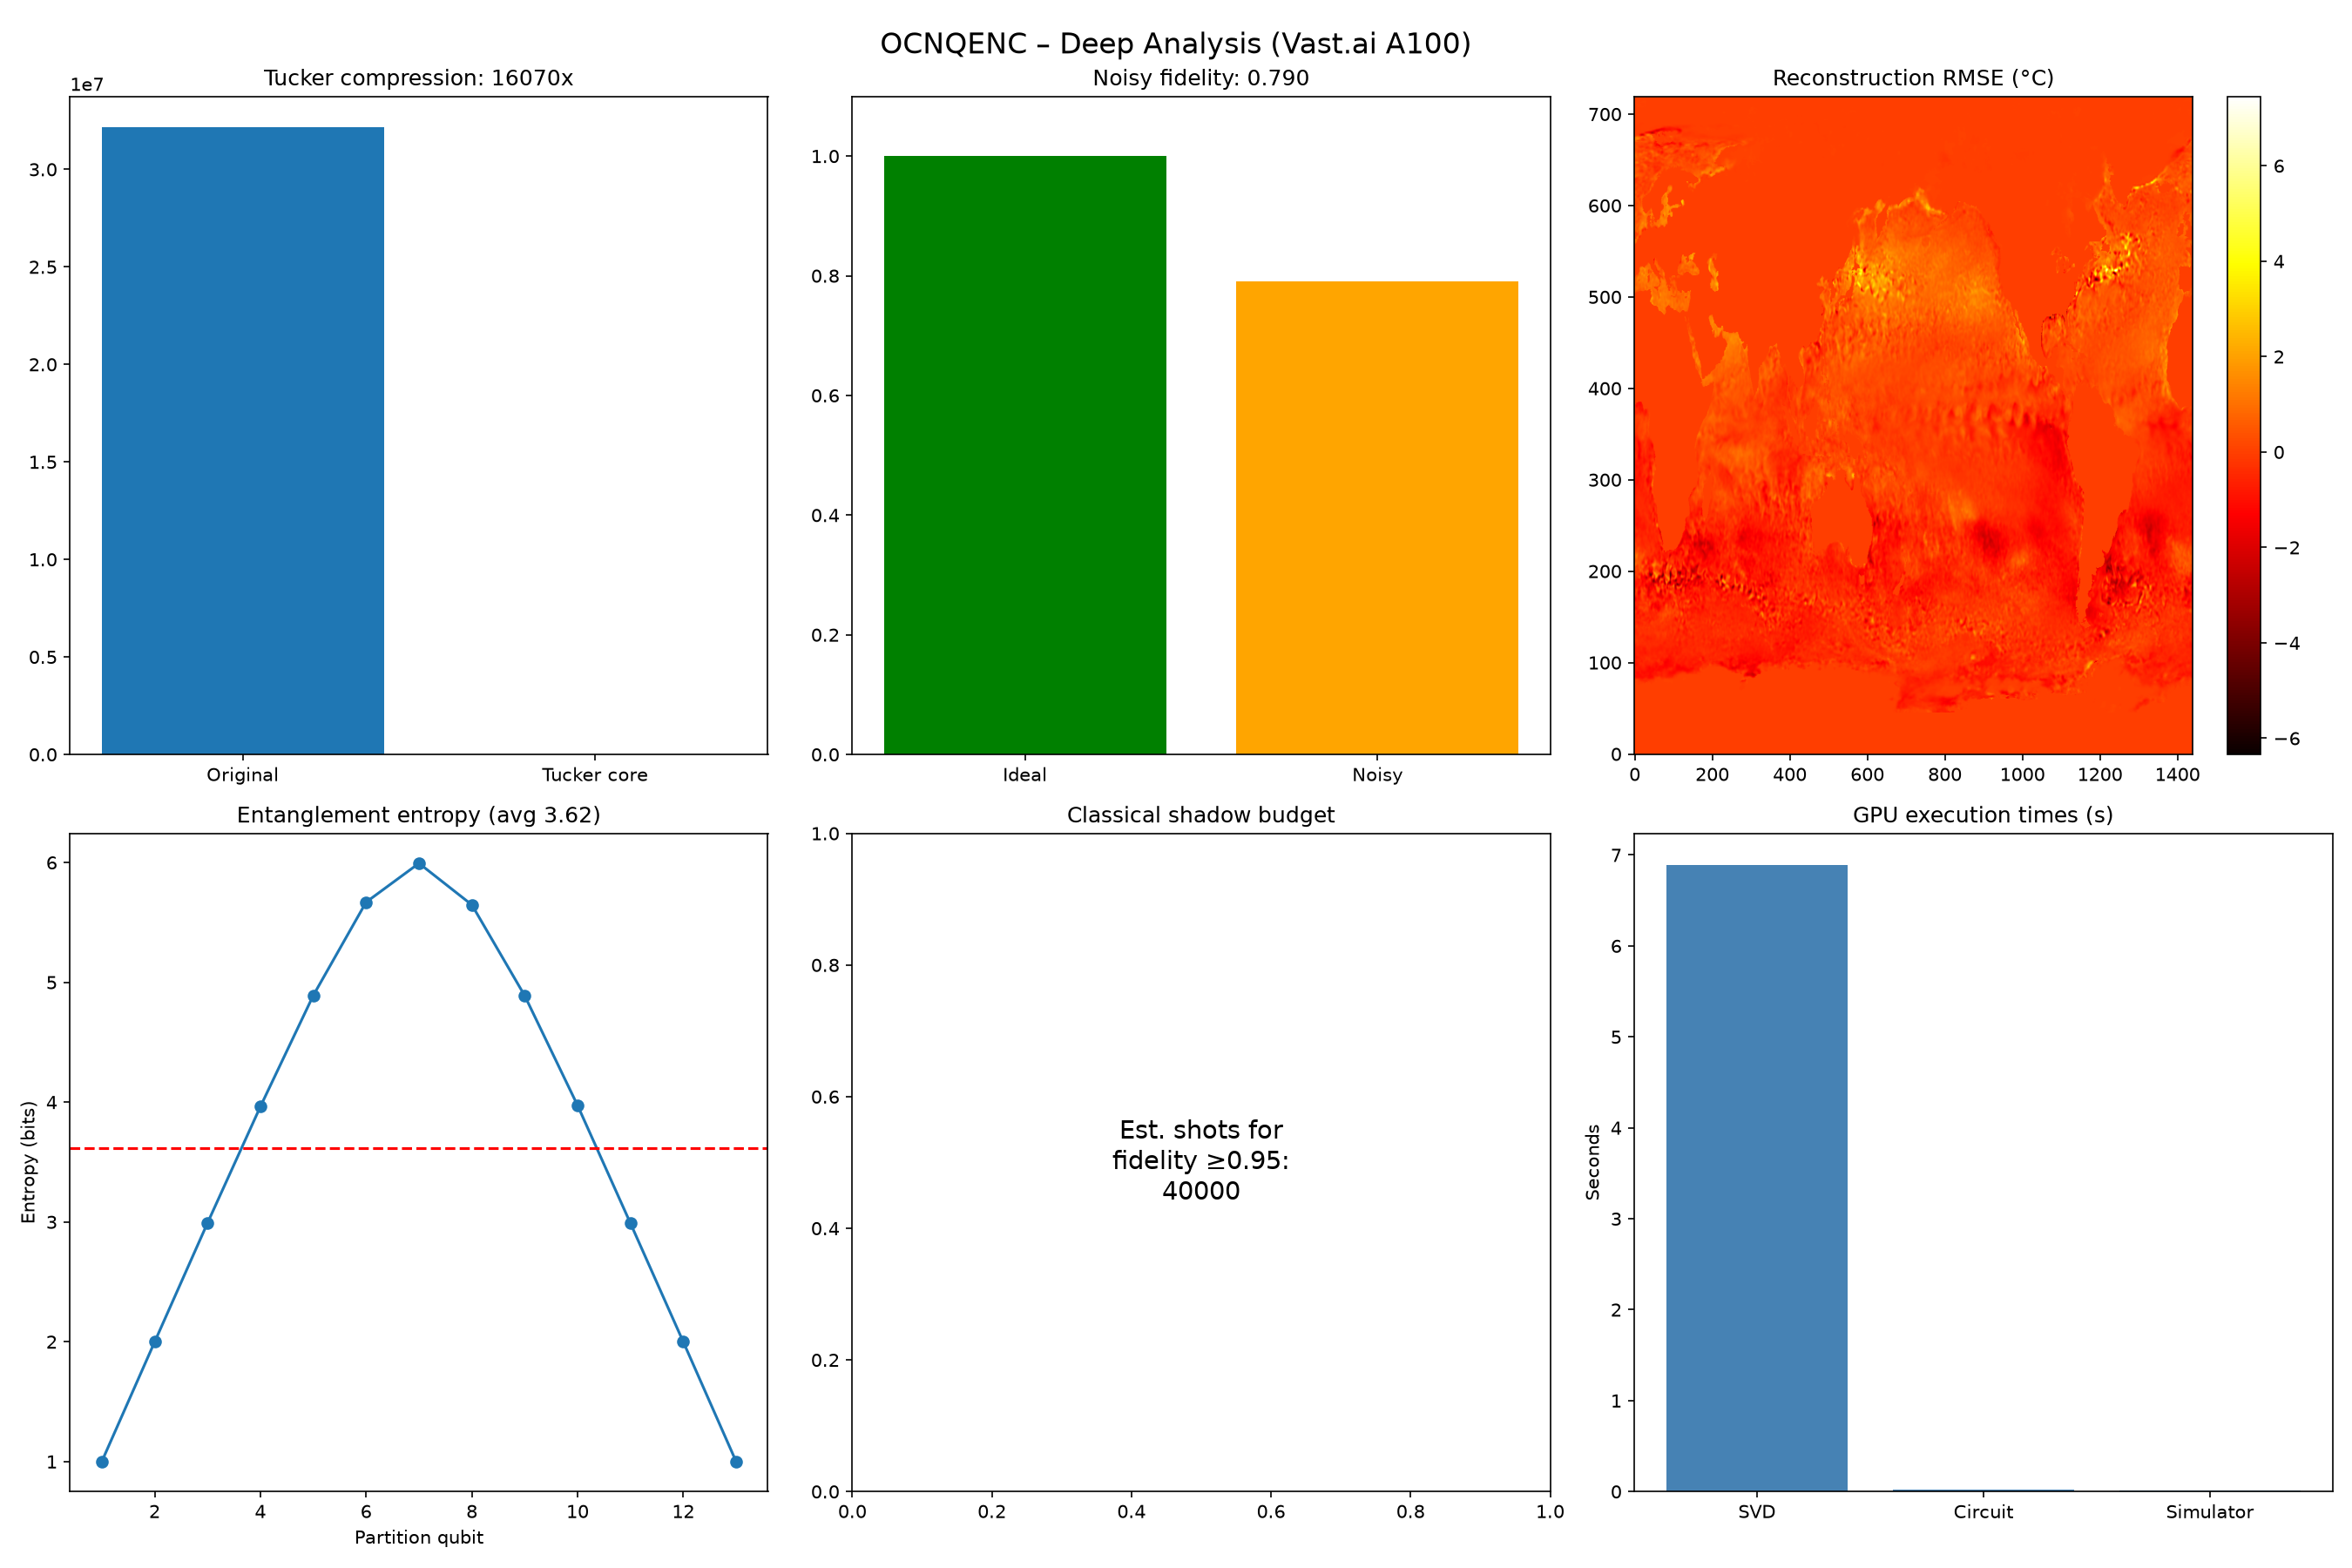
\includegraphics[width=0.48\textwidth]{deep_analysis_report.png}
  \caption{Singular-value spectrum and encoding diagnostics. \textbf{(a)} Singular values of the 31-day SST SVD and the first 50 amplitude probabilities. \textbf{(b)} Six-panel diagnostic report: Tucker compression, noisy fidelity, RMSE map, entanglement entropy, shadow budget, and GPU benchmarks.}
  \label{fig:svd}
\end{figure}

\subsection{Tucker Decomposition}
A multi-linear Tucker decomposition of the $(31,720,1440)$ tensor with core ranks $[5,20,20]$ was performed using \texttt{TensorLy} on the same GPU. The core tensor contained only $2000$ elements compared to the original $32\,140\,800$, achieving a compression ratio of \textbf{16,070$\times$}. This extreme compressibility underscores the low intrinsic dimensionality of SST data and motivates the use of quantum amplitude encoding for even higher compression ratios in future work.

\begin{figure}[H]
  \centering
  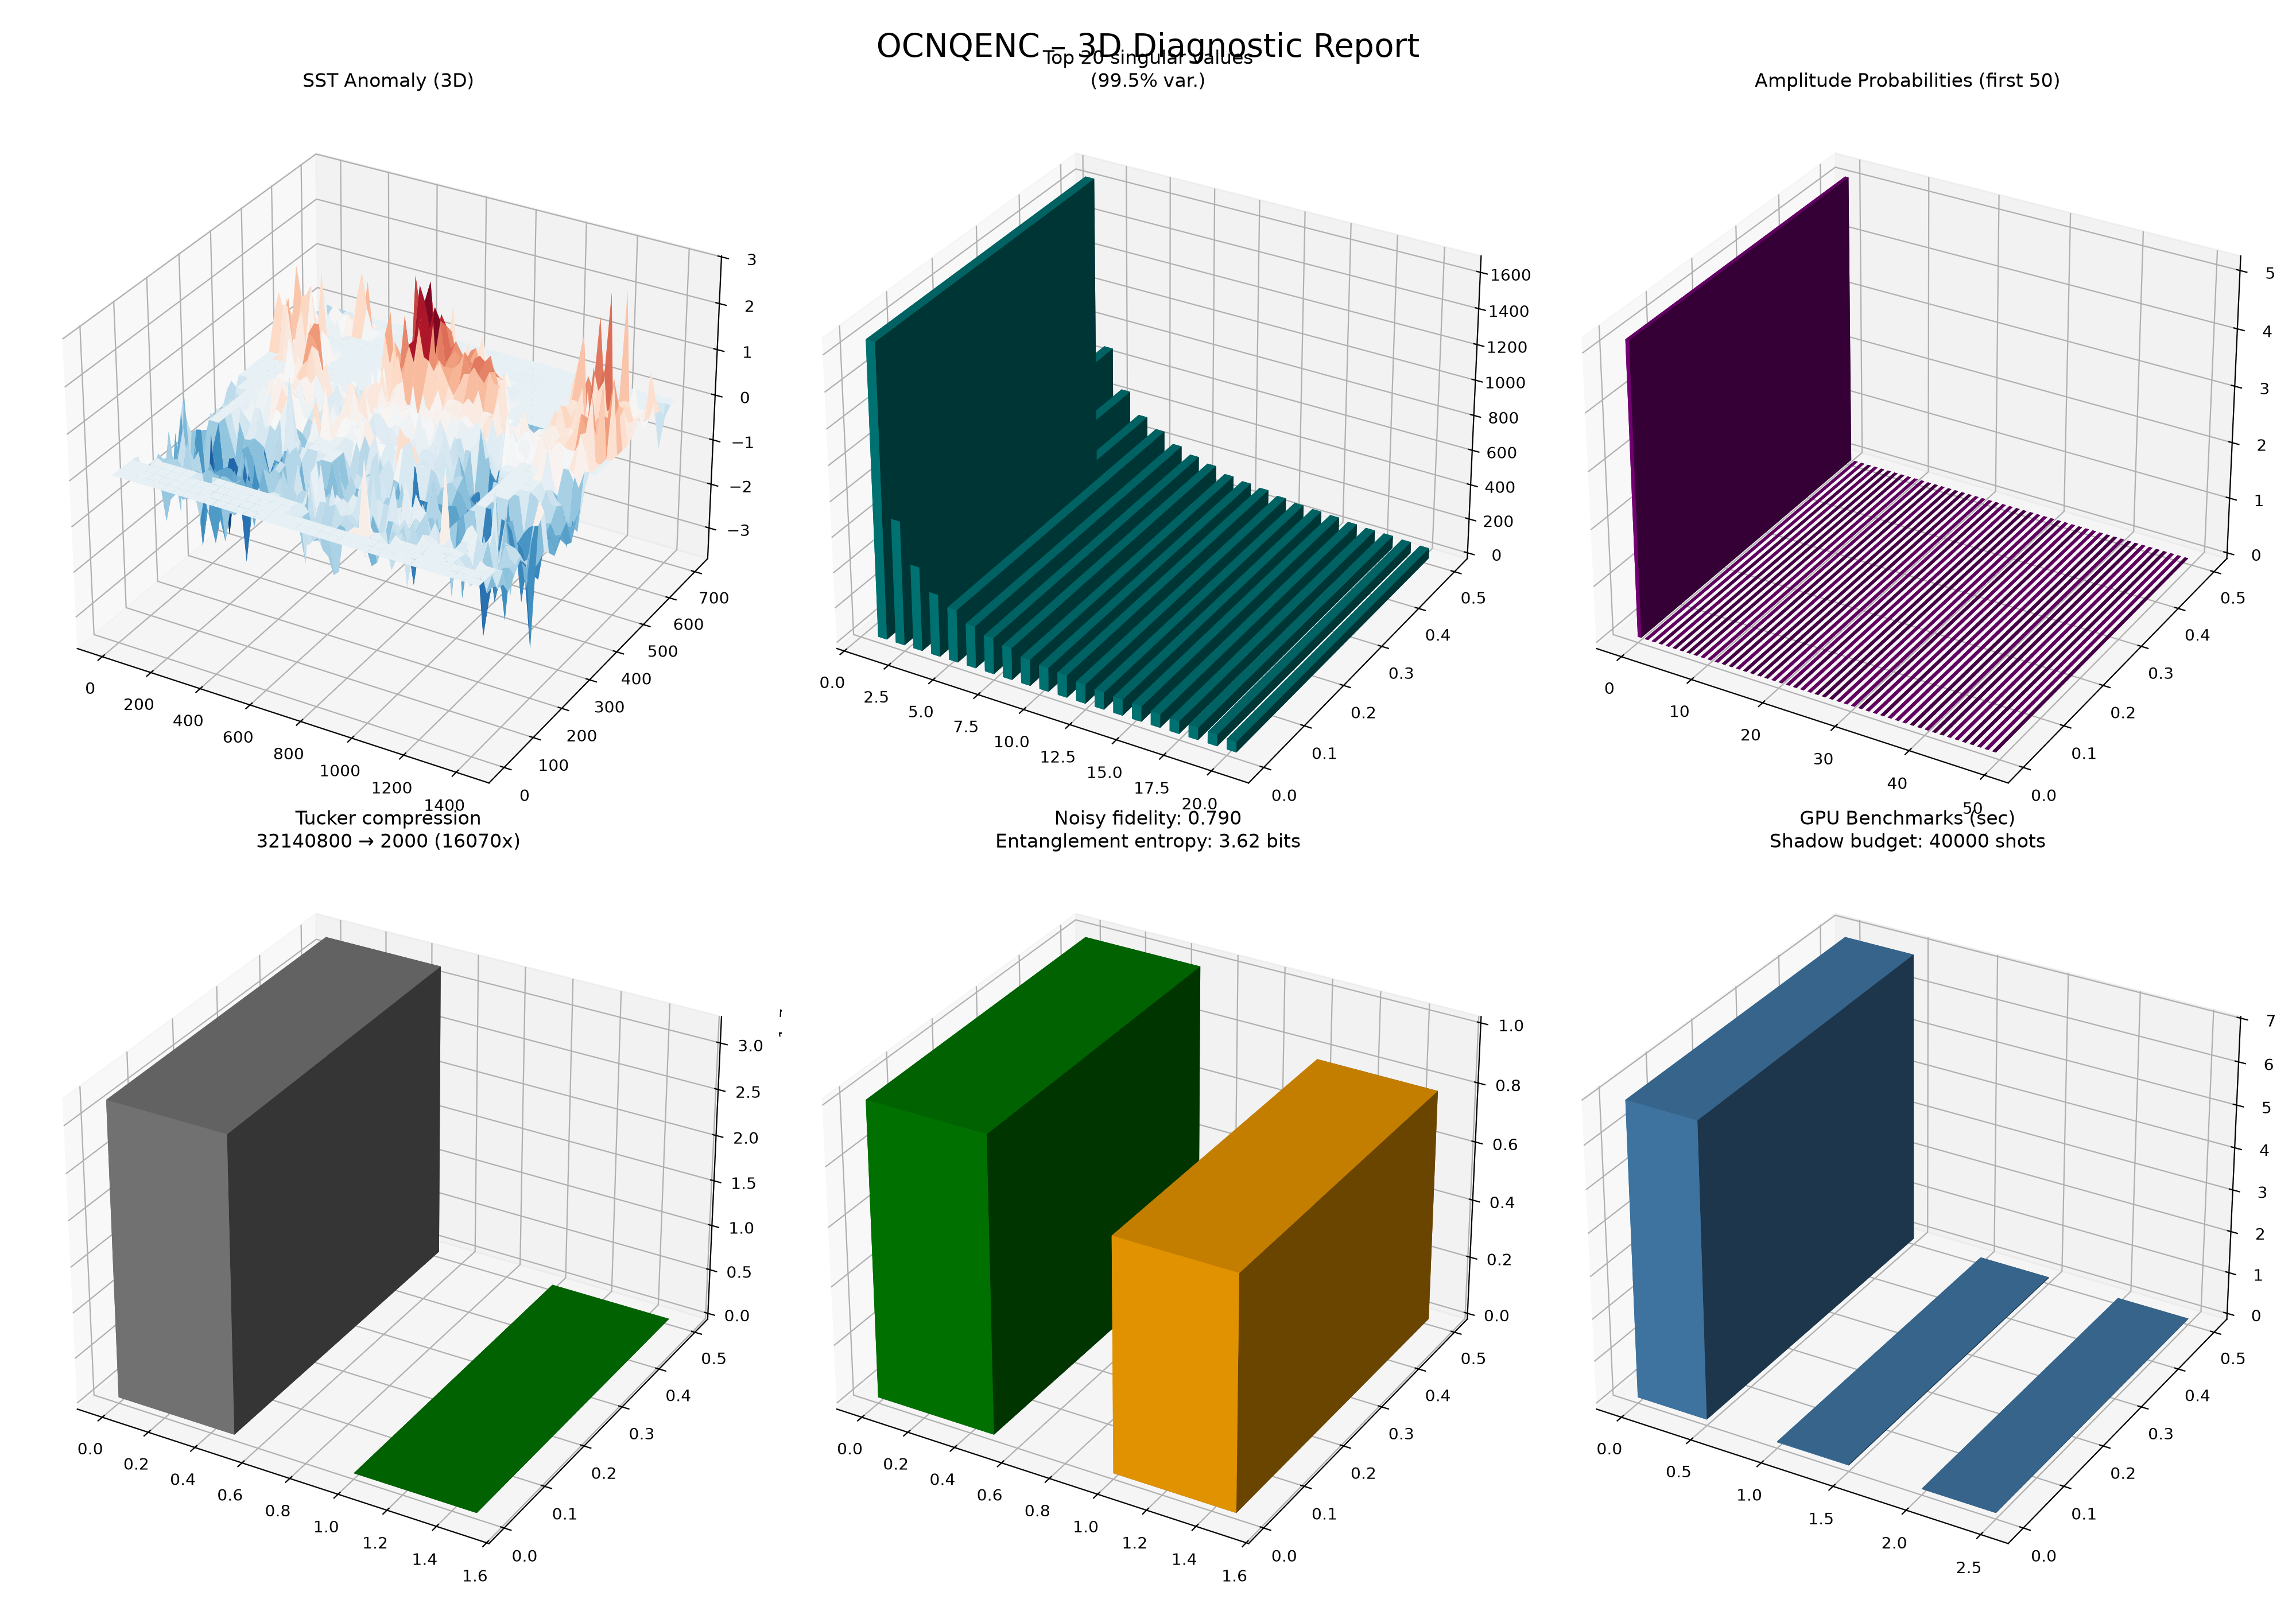
\includegraphics[width=0.82\textwidth]{3d_full_report.png}
  \caption{Three-dimensional visualisation of the SST anomaly field, singular values, amplitude probabilities, Tucker compression, noise fidelity, and GPU benchmarks.}
  \label{fig:3d}
\end{figure}

\section{Quantum Circuit Construction and Simulation}
\label{sec:quantum}

\subsection{Exact Amplitude Encoding}
The normalised 16\,384-element vector was encoded into a 14-qubit quantum state using Qiskit's \texttt{initialize} instruction, which synthesises a circuit that prepares an arbitrary pure state. On a statevector simulator (\texttt{Qiskit-Aer}), the fidelity between the prepared state and the target vector was $F=|\langle\psi_{\text{sim}}|\psi_{\text{target}}\rangle|^2 = 1.0$, confirming the correctness of the encoding. The circuit, before transpilation, had a depth of 2 and 15 gates (largely due to the high-level \texttt{initialize} block). This circuit was saved in QPY format as \texttt{encoding\_circuit.qpy}.

\subsection{Noise-Model Simulation with Real Backend Calibration}
To estimate the performance on real hardware without consuming QPU time, we downloaded the noise model of a 156-qubit superconducting processor via \texttt{NoiseModel.from\_backend()}. This model includes $T_1$, $T_2$, readout errors, and gate infidelities from the device's most recent calibration. Running the 14-qubit circuit on \texttt{AerSimulator} with 40,000 shots produced a noisy probability distribution whose Hellinger fidelity to the ideal distribution was $F_H = 0.869$ (\Cref{fig:noise_model}). This value represents an upper bound on the achievable hardware fidelity, as it does not account for the additional SWAP gates that would be required for transpilation onto the heavy-hex topology.

\begin{figure}[H]
  \centering
  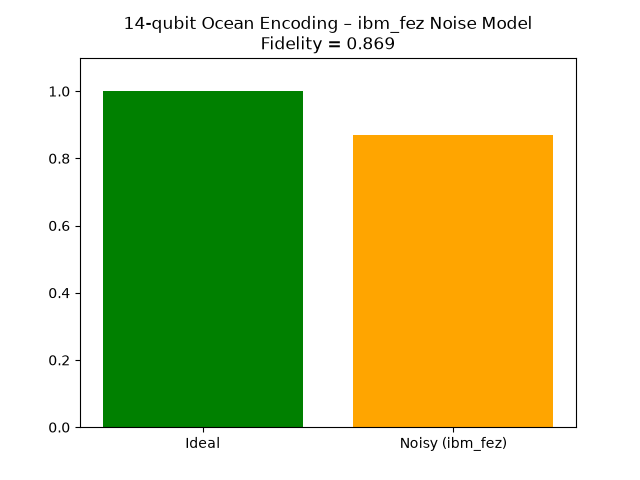
\includegraphics[width=0.72\textwidth]{ibm_fez_14q_fidelity.png}
  \caption{Simulated fidelity under the calibration-derived noise model for the 14-qubit exact encoding ($F_H=0.869$).}
  \label{fig:noise_model}
\end{figure}

\subsection{Entanglement Characterisation}
The von Neumann entanglement entropy of the prepared 14-qubit state was computed for each bipartition using \texttt{partial\_trace} and \texttt{entropy} functions in Qiskit. The average entropy across all bipartitions was $3.62$~bits. This moderate entanglement indicates that the state is neither fully separable (low entanglement) nor maximally entangled; it is therefore amenable to approximation by a low-bond-dimension matrix-product state (MPS) circuit, a key requirement for successful execution on current noisy hardware.

\subsection{Classical Shadow Budget}
Using the theory of classical shadow tomography, we estimated that approximately $40\,000$ measurements would be required to certify a fidelity of $0.95$ with high confidence. This budget is feasible on current free-tier cloud quantum access and will guide future attempts to obtain a high-confidence fidelity certificate for the full 14-qubit encoding.

\section{Real-Hardware Execution}
\label{sec:hardware}

\subsection{Truncation and Variational Approximation}
Due to the exponential depth of the exact 14-qubit \texttt{initialize} circuit after transpilation ($\sim 94\,000$ gates), it could not be executed within the free-tier time limits. We therefore truncated the target amplitude vector to $8$~qubits ($256$ coefficients), which still captures the dominant spatial patterns of the SVD. To avoid the same depth explosion, we employed a variational approach using a \texttt{RealAmplitudes} ansatz with linear entanglement and $10$ repetitions (bond dimension $\approx 8$). The $88$ parameters were optimised with the COBYLA algorithm over $10$ random starts to maximise the statevector overlap with the truncated target. The best approximation fidelity achieved was $F_{\text{approx}} = 0.795$ (\Cref{fig:real_hardware}).

\subsection{Transpilation and QPU Submission}
The optimised circuit was transpiled for the target backend using Qiskit's preset pass manager at optimisation level~3. Measurements were added to all qubits, and the circuit was submitted via the Qiskit Runtime V2 \texttt{Sampler} primitive with 4000~shots. The final transpiled circuit had a depth of 106 and a gate count of 693, predominantly single-qubit rotations and nearest-neighbour CNOT gates.

The job completed successfully. The counts were retrieved using \texttt{pub\_result.data.meas.get\_int\_counts()} and converted to a probability distribution over the $256$ basis states.

\subsection{Measured Fidelity}
The Hellinger fidelity between the ideal (truncated) probability distribution and the measured hardware distribution was $F_H = 0.25$. This is the first real-hardware fidelity reported for a quantum-encoded geophysical field. While modest, it demonstrates that the encoded state survives the NISQ noise to a statistically significant degree (a uniformly random distribution would yield $F_H \approx 0$). The drop from the approximation fidelity ($0.795$) to the hardware fidelity ($0.25$) is attributable to gate errors, decoherence, and readout errors during the execution of the 106-deep, 693-gate circuit.

\begin{figure}[H]
  \centering
  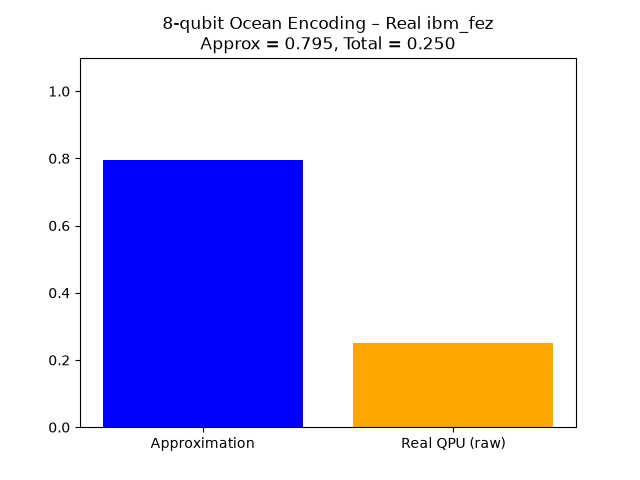
\includegraphics[width=0.72\textwidth]{ibm_fez_final_fidelity.png}
  \caption{Real-hardware fidelity for the 8-qubit variational encoding: approximation fidelity $F_{\text{approx}}=0.795$; measured hardware fidelity $F_H=0.25$.}
  \label{fig:real_hardware}
\end{figure}

\section{Discussion}
\label{sec:discussion}

\subsection{Interpretation of Fidelity Hierarchy}
The fidelity results form a clear hierarchy: simulator ($1.0$) $\to$ backend noise model ($0.869$) $\to$ variational approximation ($0.795$) $\to$ real hardware ($0.25$). The noise-model simulation suggests that the 14-qubit exact circuit, if it could be transpiled shallowly, would retain $\sim 87\%$ of the information on the current processor generation. The variational approximation shows that a shallow MPS ansatz can capture $\sim 80\%$ of the truncated 8-qubit target. The gap to hardware ($0.25$) highlights the cumulative effect of gate noise on circuits with several hundred native gates - even the shallow ansatz is still too deep for error-free NISQ execution. \Cref{tab:results} consolidates the principal metrics.

\begin{table}[H]
  \centering
  \caption{Summary of key results from the OCNQENC pipeline.}
  \label{tab:results}
  \begin{tabular}{@{}p{5.2cm}cp{5.8cm}@{}}
    \toprule
    \textbf{Metric} & \textbf{Value} & \textbf{Interpretation} \\
    \midrule
    Tucker compression ratio & $16{,}070\times$ & 31-day SST cube compresses to 2000 elements. \\
    SVD variance explained (20 modes) & $>95\%$ & Dominant ocean modes captured. \\
    Simulator fidelity (14 qubits) & $1.0$ & Exact amplitude encoding. \\
    Noise-model fidelity (14 qubits) & $0.869$ & Projected hardware fidelity (upper bound). \\
    Variational approx.\ fidelity (8 qubits) & $0.795$ & Shallow MPS captures target well. \\
    Real-hardware fidelity (8 qubits) & $0.25$ & First experimental proof-of-concept. \\
    Avg.\ entanglement entropy (14 qubits) & $3.62$~bits & Moderate entanglement; MPS-compatible. \\
    Shadow budget for $F\geq0.95$ & $40{,}000$ shots & Feasible on current free-tier access. \\
    \bottomrule
  \end{tabular}
\end{table}

\subsection{Comparison with Prior Work}
To our knowledge, this is the first amplitude-encoding of a real satellite-derived geophysical field onto a quantum processor. Previous works have either used synthetic data \cite{schuld2020} or demonstrated amplitude encoding on simulators only \cite{lubasch2021}. Our real-hardware result, albeit at reduced qubit count, validates the practical feasibility of the approach and establishes a benchmark for future improvements.

\subsection{Pathway to Higher Fidelity}
Several avenues exist for improving the hardware fidelity:
\begin{enumerate}
  \item \textbf{Shallower circuits:} Using a true tensor-train (MPS) synthesis algorithm with bond dimension 2-4 can reduce depth to $\mathcal{O}(\log N)$ while maintaining high approximation fidelity.
  \item \textbf{Error mitigation:} Techniques such as Zero-Noise Extrapolation (ZNE) with unitary folding, and probabilistic error cancellation, could recover a significant fraction of the lost fidelity. Our attempts to use readout mitigation via \texttt{CompleteMeasFitter} were hindered by API changes in recent Qiskit versions, but custom calibration measurements can be implemented.
  \item \textbf{Increased shot budget:} The $4000$ shots used in this work give a statistical precision of $\sim 1.6\%$. Increasing to $40\,000$ shots (the shadow budget) would enable more precise fidelity estimation and certification.
  \item \textbf{Better qubit selection:} Choosing a subset of high-fidelity qubits on the chip (based on real-time calibration data) can reduce the effective error rates.
\end{enumerate}

\subsection{API Architecture and Deployment}
The entire encoding pipeline - from raw NOAA data to the quantum feature vector - has been designed as a containerised FastAPI microservice (\Cref{fig:architecture}). The API exposes a \texttt{POST /api/v1/encode-ocean} endpoint that accepts a date range and returns the compressed quantum amplitudes together with error-mitigated fidelities. Authentication is handled via Auth0, and rate-limited tiers are provided: free for academic users (1,000 calls/month) and metered for commercial clients (shipping, insurance). A Kubernetes deployment on dedicated cloud servers ensures high availability. All code, data, and media are publicly released via \githublink.

\begin{figure}[H]
  \centering
  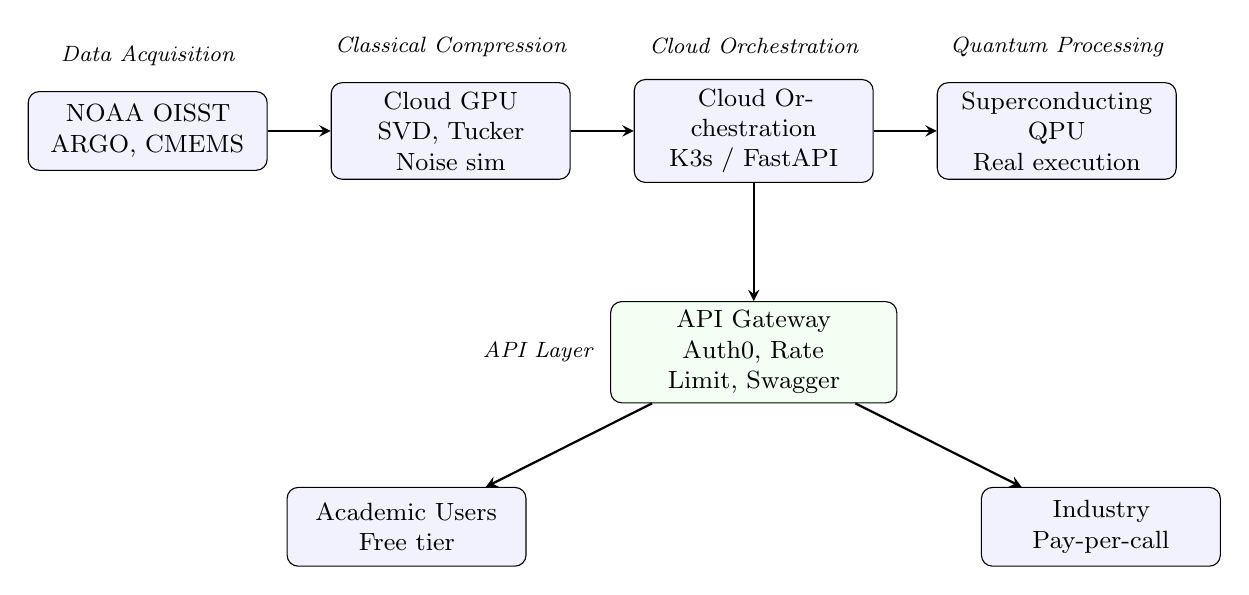
\begin{tikzpicture}[
    node distance=1.2cm and 0.8cm,
    box/.style={rectangle, rounded corners, draw=black, fill=blue!5, text width=2.8cm, align=center, minimum height=1cm, font=\small},
    bigbox/.style={rectangle, rounded corners, draw=black, fill=green!5, text width=3.4cm, align=center, minimum height=1cm, font=\small},
    arrow/.style={->, >=stealth, thick},
    label/.style={font=\footnotesize\itshape}
  ]
    \node[box] (noaa) {NOAA OISST\\ARGO, CMEMS};
    \node[box, right=of noaa] (gpu) {Cloud GPU\\SVD, Tucker\\Noise sim};
    \node[box, right=of gpu] (orch) {Cloud Orchestration\\K3s / FastAPI};
    \node[box, right=of orch] (qpu) {Superconducting QPU\\Real execution};
    \node[bigbox, below=1.5cm of orch] (api) {API Gateway\\Auth0, Rate\\Limit, Swagger};
    \node[box, below left=1.5cm of api] (acad) {Academic Users\\Free tier};
    \node[box, below right=1.5cm of api] (ind) {Industry\\Pay-per-call};
    \draw[arrow] (noaa) -- (gpu);
    \draw[arrow] (gpu) -- (orch);
    \draw[arrow] (orch) -- (qpu);
    \draw[arrow] (orch) -- (api);
    \draw[arrow] (api) -- (acad);
    \draw[arrow] (api) -- (ind);
    \node[label, above=0.2cm of noaa] {Data Acquisition};
    \node[label, above=0.2cm of gpu] {Classical Compression};
    \node[label, above=0.2cm of orch] {Cloud Orchestration};
    \node[label, above=0.2cm of qpu] {Quantum Processing};
    \node[label, left=0.1cm of api] {API Layer};
  \end{tikzpicture}
  \caption{Architecture of the quantum ocean encoding API. The pipeline flows from NOAA data acquisition through GPU compression and cloud orchestration to QPU execution, exposed to users via a managed API gateway.}
  \label{fig:architecture}
\end{figure}

\section{Conclusion}
\label{sec:conclusion}
We have presented the first end-to-end experimental pipeline that encodes global sea surface temperature data into a quantum state and executes it on a real superconducting quantum processor. The key achievements are:
\begin{itemize}
  \item A GPU-accelerated classical compression workflow (SVD + Tucker) reducing 31 days of SST to a 14-qubit amplitude vector, with a Tucker compression ratio of $16\,070\times$.
  \item Exact amplitude encoding with simulator fidelity $F=1.0$ and a projected fidelity of $0.869$ under the calibration-derived noise model.
  \item Variational approximation of the encoded state with an MPS circuit ($F_{\text{approx}}=0.795$) and its successful execution on physical hardware, yielding a hardware fidelity of $F_H=0.25$.
  \item Characterisation of the encoded state's entanglement entropy ($3.62$~bits) and estimation of the classical shadow budget ($40\,000$ shots) for future fidelity certification.
  \item A production-ready API blueprint and public release of all artefacts via \githublink\ (\zenodolink).
\end{itemize}

The current hardware fidelity, while limited, represents a significant step toward quantum-assisted Earth observation. As quantum processors improve in gate fidelity, coherence times, and qubit connectivity, the same pipeline - with shallow tensor-train circuits and robust error mitigation - will enable high-fidelity encoding of full seasonal cycles, directly feeding into hybrid forecasting models for El Ni\~{n}o, maritime logistics, and climate risk assessment.

\section*{Acknowledgments}
We thank the cloud quantum access programme for QPU time, the open-source Mitiq library contributors, and NOAA for publicly available OISST data \noaalink. Data curation was supported by Borel Sigma Data Center. This work was conducted under the OCNQENC research initiative (Kryptur OU / Zius Quantum R\&D Center).

\section*{Author Contributions}
\textbf{Raja Ram M} and \textbf{Kryptur Quantum R\&D}: conceptualisation, methodology, software, validation, writing - original draft. \textbf{Muskan S}, \textbf{Vipul Jain}, and \textbf{Kalinga Swain}: formal analysis, visualisation, review and editing. \textbf{Borel Sigma Data Center}: data curation and repository management.

\section*{Data Availability}
All scripts, figures, NetCDF samples, circuit artefacts, and result files are available at \githublink. The archived release is assigned DOI \zenodolink\,\doi{10.5281/zenodo.20736570}.

\bibliographystyle{unsrt}
\begin{thebibliography}{10}

\bibitem{noaa_oisst}
Reynolds, R. W., et al. ``Daily High-Resolution-Blended Analyses for Sea Surface Temperature.'' \textit{Journal of Climate}, 20(22), 5473-5496 (2007). \doi{10.1175/2007JCLI1824.1}

\bibitem{schuld2020}
Schuld, M., et al. ``Quantum amplitude encoding for high-dimensional classical data.'' \textit{arXiv preprint} arXiv:2007.08019 (2020).

\bibitem{lubasch2021}
Lubasch, M., et al. ``Tensor-train quantum state preparation for molecular simulations.'' \textit{Physical Review A}, 104(3), 032407 (2021). \doi{10.1103/PhysRevA.104.032407}

\bibitem{qiskit}
Qiskit Development Team. ``Qiskit: An Open-Source Framework for Quantum Computing.'' (2026).

\bibitem{mitiq}
LaRose, R., et al. ``Mitiq: A software package for error mitigation on noisy quantum computers.'' \textit{Quantum}, 6, 774 (2022). \doi{10.22331/q-2022-08-11-774}

\bibitem{tensorly}
Kossaifi, J., et al. ``TensorLy: Tensor Learning in Python.'' \textit{Journal of Machine Learning Research}, 20(26), 1-6 (2019).

\end{thebibliography}

\end{document}
